\chapter{Experimental Results}
\label{chap:results}
\section{Experimental Methodology}


%Add the introduction sentence, we compare so-and-so with standard MAUT
We use two standard datasets, \textbf{Camera} and \textbf{PC}, in our experiments.
Both the datasets are available for download at \cite{datasets}.
Cases with missing values have been removed from the datasets.
After removing the cases with missing values, the Camera dataset contains 173 cameras with 10 attributes and the PC dataset contains 120 PCs with 8 attributes.
A typical PC in the PC dataset is shown in Table \ref{tab:pc} and a typical camera in the Camera dataset is shown in Table \ref{tab:camera}.


\begin{table}
\caption{A typical PC in the PC dataset}
\centering
\renewcommand{\arraystretch}{1.2}
\label{tab:pc}

\begin{tabular}{|l|l|}
\hline
Manufacturer & Apple \\
\hline
Processor Type & PowerPC G3 \\
\hline
Processor Speed(MHz) & 600 \\
\hline
Monitor (Inches) & 15 \\
\hline
Type & Laptop \\ 
\hline
RAM (MB) & 512 \\
\hline
Drive Capacity(GB) & 40 \\
\hline
Price (\$) & 986\\
\hline
\end{tabular}
\end{table}

\begin{table}
\caption{A typical camera in the Camera dataset}
\centering
\renewcommand{\arraystretch}{1.2}
\label{tab:camera}

\begin{tabular}{|l|l|}
\hline
Manufacturer & Sony \\
\hline
Model & DSC-T11 \\
\hline
Price(\$) & 383\\
\hline
Format & Ultra-compact\\
\hline
Resolution (MP)  &5\\
\hline
Optical Zoom (X) &3 \\
\hline
Digital Zoom (X) &4\\
\hline
Weight (grams) &230\\
\hline
Storage Type & Memory Stick\\
\hline
Storage Included (MB)& 32\\
\hline
\end{tabular}
\end{table}

To evaluate the algorithms in offline setting, we simulate an artificial user who interacts with the recommender system.
A product is first selected from the case base and a random subset of it's features is used to formulate the simulated user's query at the beginning of the recommendation session.
This product is now the target for the recommender system and the recommendation session terminates when this product appears in the list of $K$ products shown to the user. 
Subsets of 1, 3 and 5 features are referred to as Q1, Q3 and Q5 respectively.
Queries in Q1 category correspond to users who have very limited domain knowledge.
Queries in Q5 category correspond to users who have a very clear idea about what products they exactly want.
For both PC and Camera datasets, we generate queries of the type Q1, Q3 and Q5.
The same set of queries has been used for all the experiments done below.
Each product in the case-base is set as the target product 10 times and this is repeated for all products in the case-base.
Hence a total of 1730 and 1200 queries for each of the three categories Q1, Q3 and Q5 have been generated for Camera and PC datasets respectively.
The evaluation of all the algorithms described in Sections \ref{sec:div} to \ref{sec:additive} are performed in two scenarios described in Section \ref{sec:focus} and \ref{sec:noisy}, where the artifical user interacts with the system in two different ways.
The complete implementation for all the algorithms described in Sections \ref{sec:div} to \ref{sec:additive} is available at 
%\url{https://github.com/abharath27/MAUTNew}.
\cite{implementation}.

\section{Highly Focused/Optimal Framework}
\label{sec:focus}
Evaluation in Highly Focused Recommendation Framework is the same way of evaluation described in Section \ref{sec:offline}.
In this scenario we assume that the user is relatively sure of his preferences and hence chooses the critique string that is maximally compatible with the target product in each cycle.
The notion of selecting the most compatible critique string is shown in Figure \ref{fig:focus}

%This will help  us to illustrate the noisy framework better.
\begin{figure}[h]
  \centering
  \captionsetup{justification=centering}
    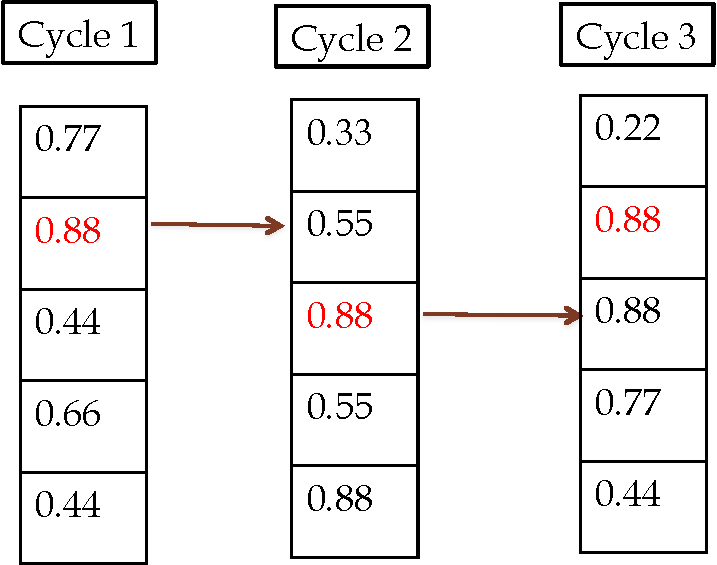
\includegraphics[width=0.5\textwidth]{figures-bharath/focus.pdf}
  \caption{Numbers in the boxes represent the compatibilities of each of the five critique strings with the target product. Simulated user selects the most compatible critique string (red) in each cycle.}
\label{fig:focus}
\end{figure}

\begin{figure}[h]
  \centering
  \captionsetup{justification=centering}
    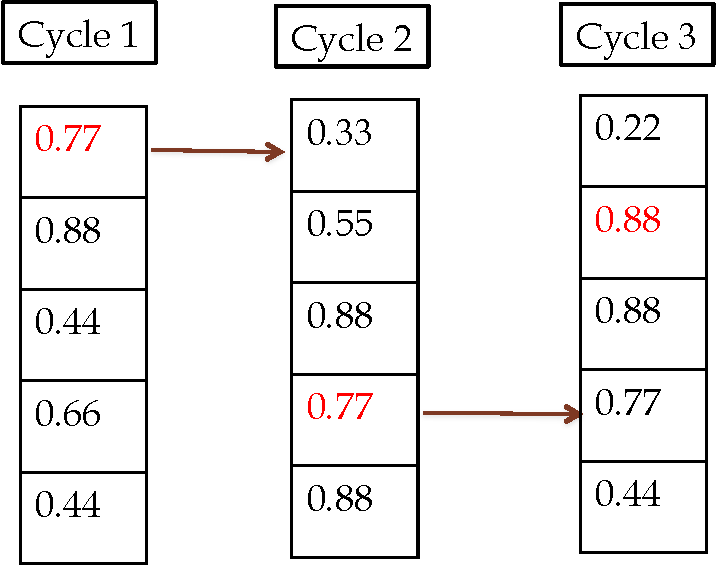
\includegraphics[width=0.5\textwidth]{figures-bharath/noisy.pdf}
  \caption{Simulated user selects sub-optimal critique strings due to the introduction of noise}
\label{fig:noisy}
\end{figure}

\section{Noisy Framework}
\label{sec:noisy}
In this scenario, the simulated user does not select the most optimal critique string during each cycle.
This kind of evaluation is similar to the evaluation procedure described in \cite{suggestion}.
Noise is introduced into the process by varying the compatibility scores of the critique strings within some threshold. 
In our experiments, we have used a noise level of 10\%, i.e, the compatiblity scores can be changed by upto +/-10\% of their actual values.
Due to the introduction of noise, the user makes sub-optimal choices in each cycle as shown in Figure \ref{fig:noisy}.
In the experiments, the simulated user selects a sub-optimal critique string for 28\% times on an average in noisy setting.
The average number of interaction cycles in this scenario is slightly higher in this scenario compared to the number of cycles in highly focused recommendation framework because of sub-optimal choices made by the simulated user.


\section{Results}
\subsection{Diversity enhancing algorithms(DIV, DIV2)}
\label{sec:div_results}
The algorithm DIV, described in Section \ref{sec:div} introduces diversity among critique strings in every cycle. 
DIV2, described in Section \ref{sec:div2}, varies the level of diveristy in critique strings according to the extent to which the user's preferences have stabilized.
The results for the algorithms DIV and DIV2 in both optimal and noisy settings for PC and Camera datasets are summarized in Figures \ref{fig:div_camera_opt} to \ref{fig:div_pc_noisy}.
For the queries of category Q1 on the in Figure \ref{fig:div_camera_opt}, the implementation of standard MAUT based recommendation takes 9.21 cycles on an average to reach a target product.
DIV and DIV2 take 7.82 and 6.82 cycles on an average to reach the target product.
DIV and DIV2 achieve an average reduction of 22.6\% and 27.9\% respectively in the average number of interaction cycles in optimal setting for the camera dataset.
The average number of cycles taken by MAUT to reach the target product is 10.35 in noisy setting, which is 12\% higher than the number of cycles in the optimal setting.
DIV and DIV2 achieve an average improvement of 29.5\% and 39.8\% respectively in noisy setting for the camera dataset, which is higher than the reductions achieved in optimal setting.
The results of the improvements achieved by various algorithms is summarized in Table \ref{tab:summary}.
We can see from the table that most algorithms achieve a higher improvement in noisy setting than in optimal setting.



\begin{figure}[h]
\centering
\begin{minipage}{.45\textwidth}
  \centering
  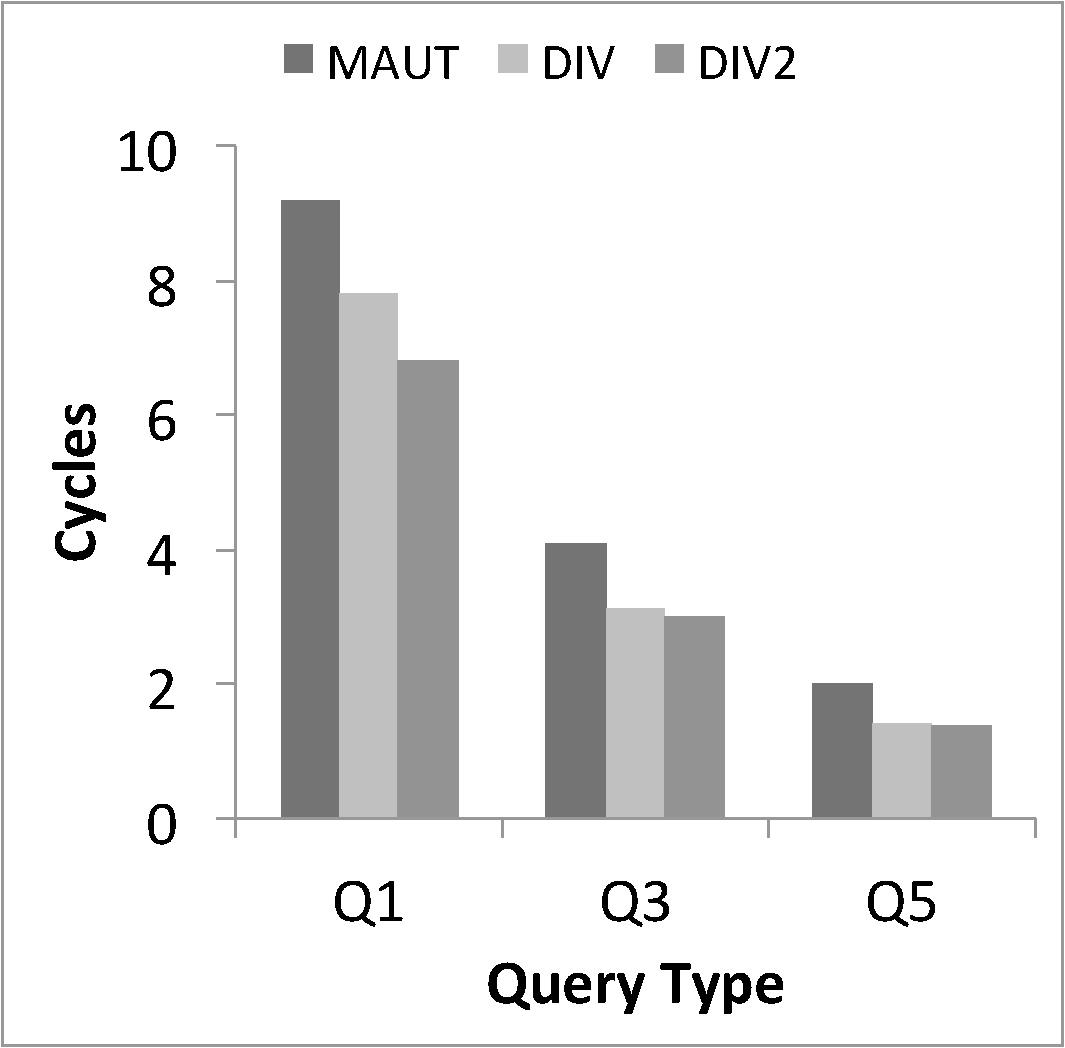
\includegraphics[width=1\linewidth]{figures-bharath/div_camera_opt}
  \caption[]{Average number of interaction cycles on Camera dataset - optimal user model}
  \label{fig:div_camera_opt}
\end{minipage}%
\;\;\;\;\;\;
\begin{minipage}{.45\textwidth}
  \centering
  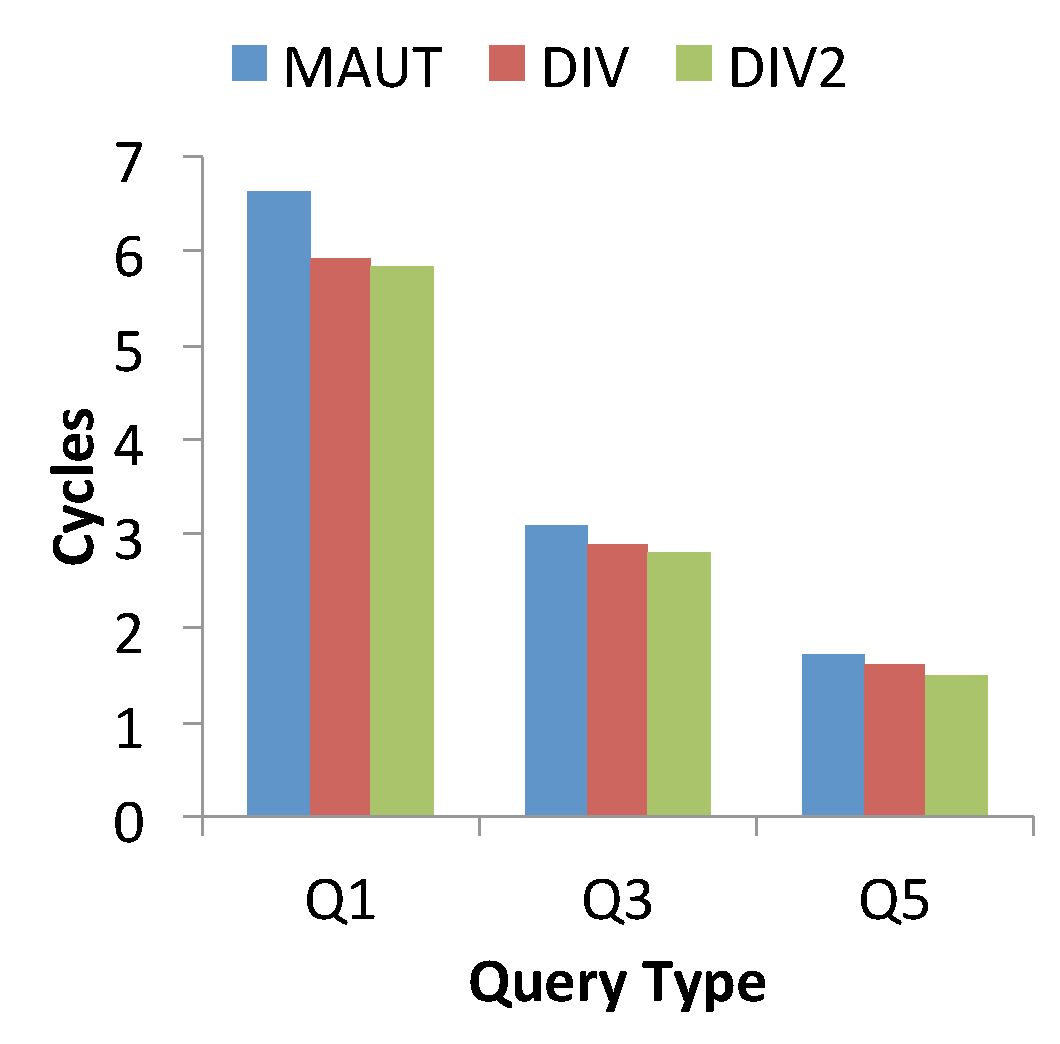
\includegraphics[width=1\linewidth]{figures-bharath/div_pc_opt}
  \caption[]{Average number of interaction cycles on PC dataset - optimal user model}
  \label{fig:div_pc_opt}
\end{minipage}
\end{figure}

\begin{figure}[h]
\centering
\begin{minipage}{.45\textwidth}
  \centering
  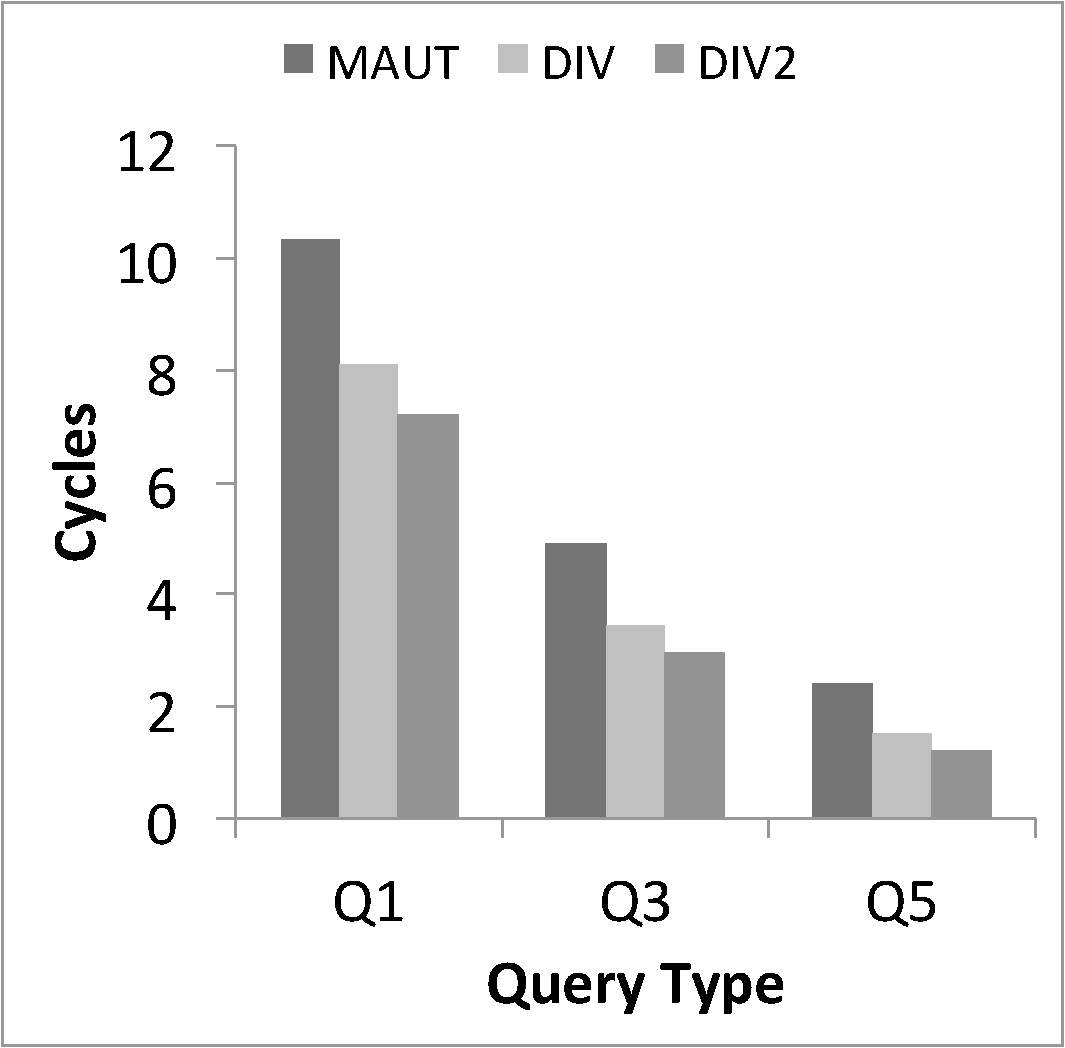
\includegraphics[width=1\linewidth]{figures-bharath/div_camera_noisy}
  \caption[]{Average number of interaction cycles on Camera dataset - noisy framework}
  \label{fig:div_camera_noisy}
\end{minipage}%
\;\;\;\;\;\;
\begin{minipage}{.45\textwidth}
  \centering
  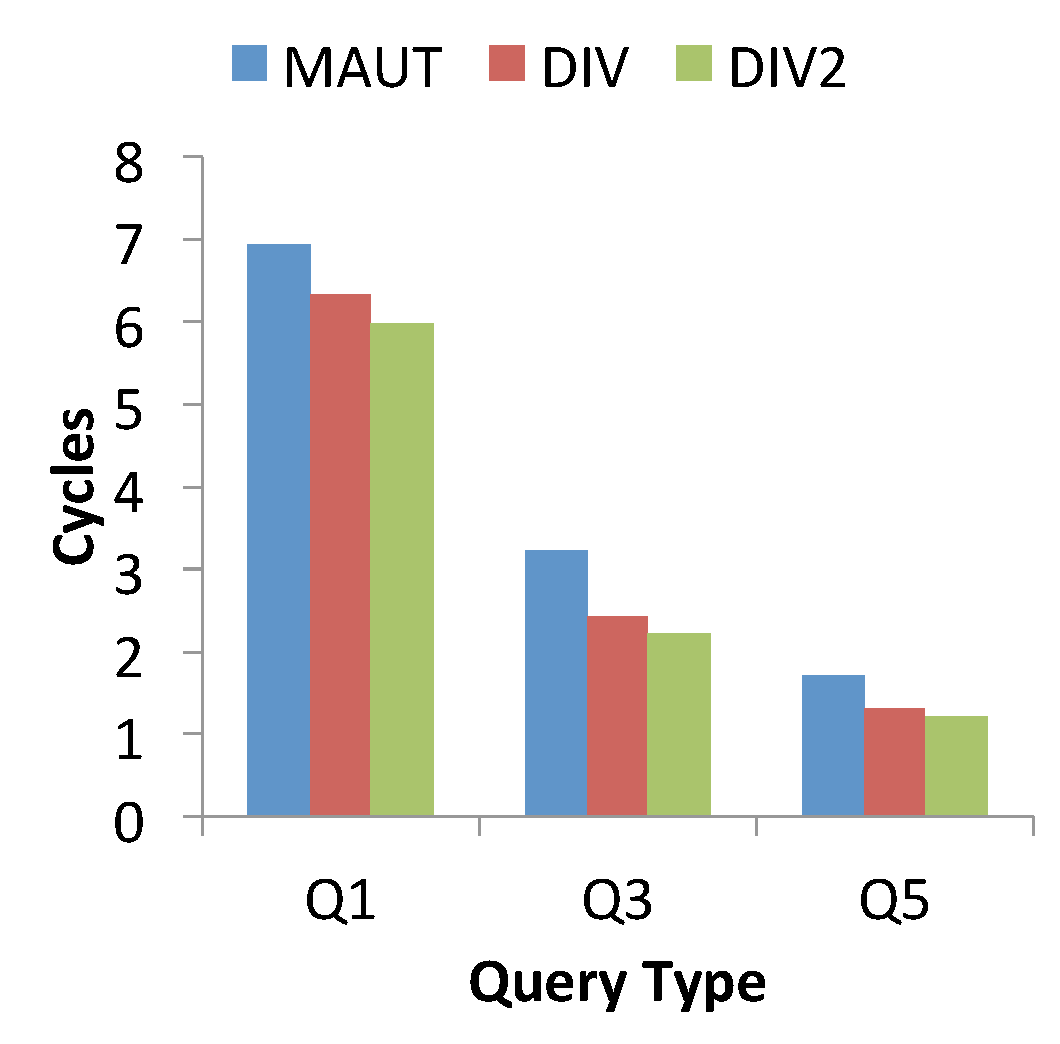
\includegraphics[width=1\linewidth]{figures-bharath/div_pc_noisy}
  \caption[]{Average number of interaction cycles on PC dataset - noisy framework}
  \label{fig:div_pc_noisy}
\end{minipage}
\end{figure}

\subsection{Algorithms that combine similarity with utility(ADDPREF, ADDPREF2, SIM)}
ADDPREF, described in Section \ref{sec:addTerm} promotes products that have a critique pattern similar to the product selected by the user in previous cycle.
ADDPREF2, described in Section \ref{sec:addTerm} is an extension to ADDPREF, where we consider critique overlap of a product with all the products that have been selected so far.
The results for both the algorithms are summarized in Figures \ref{fig:addPref_camera_opt} to \ref{fig:addPref_pc_noisy}.
In optimal framework, ADDPREF and ADDPREF2 give an average improvement of 29.1\% and 33.7\% respectively on the camera dataset.
The results for other evaluation settings have given in Table \ref{tab:summary}.

\begin{figure}[h]
\centering
\begin{minipage}{.45\textwidth}
  \centering
  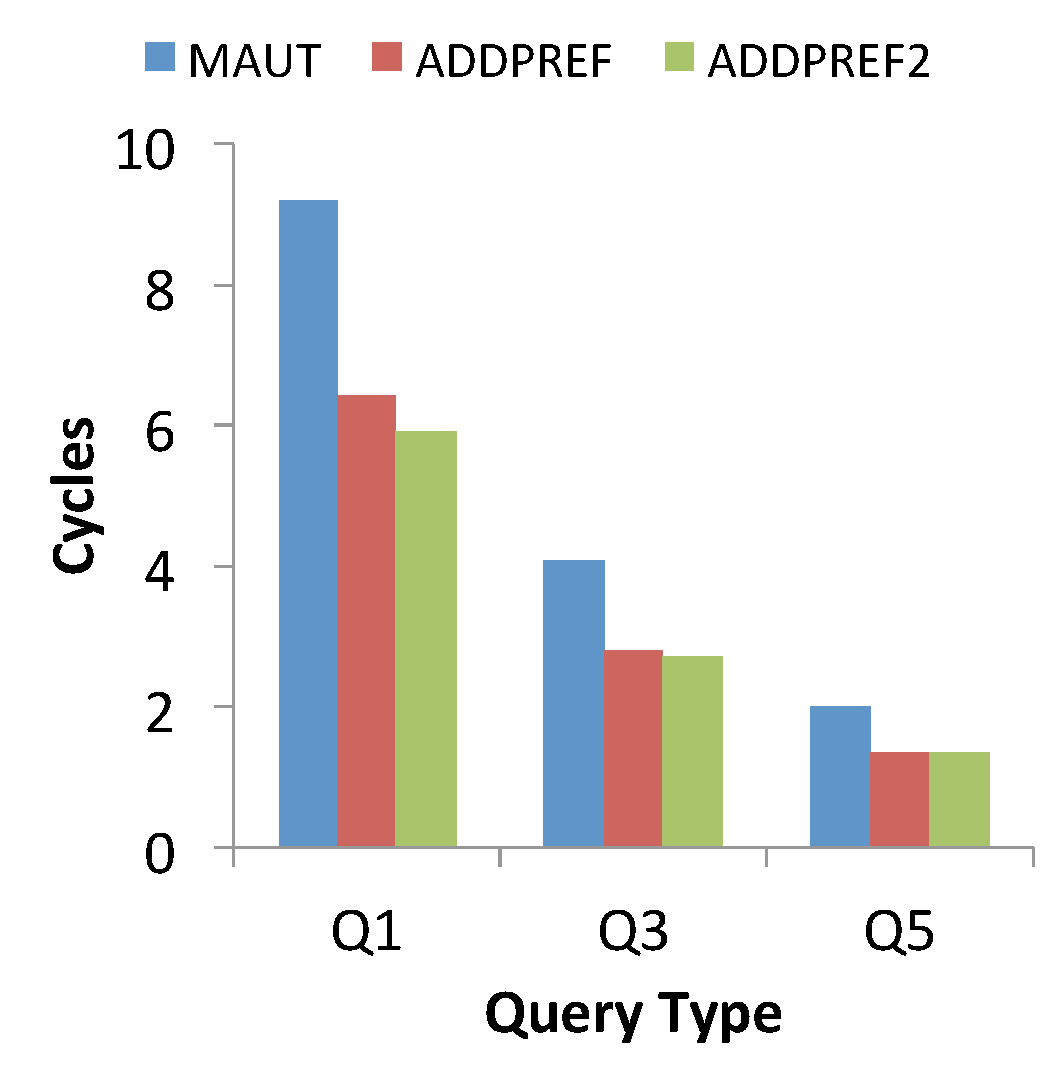
\includegraphics[width=1\linewidth]{figures-bharath/addPref_camera_opt}
  \caption[]{Average number of interaction cycles on Camera dataset - optimal user model}
  \label{fig:addPref_camera_opt}
\end{minipage}%
\;\;\;\;\;\;
\begin{minipage}{.45\textwidth}
  \centering
  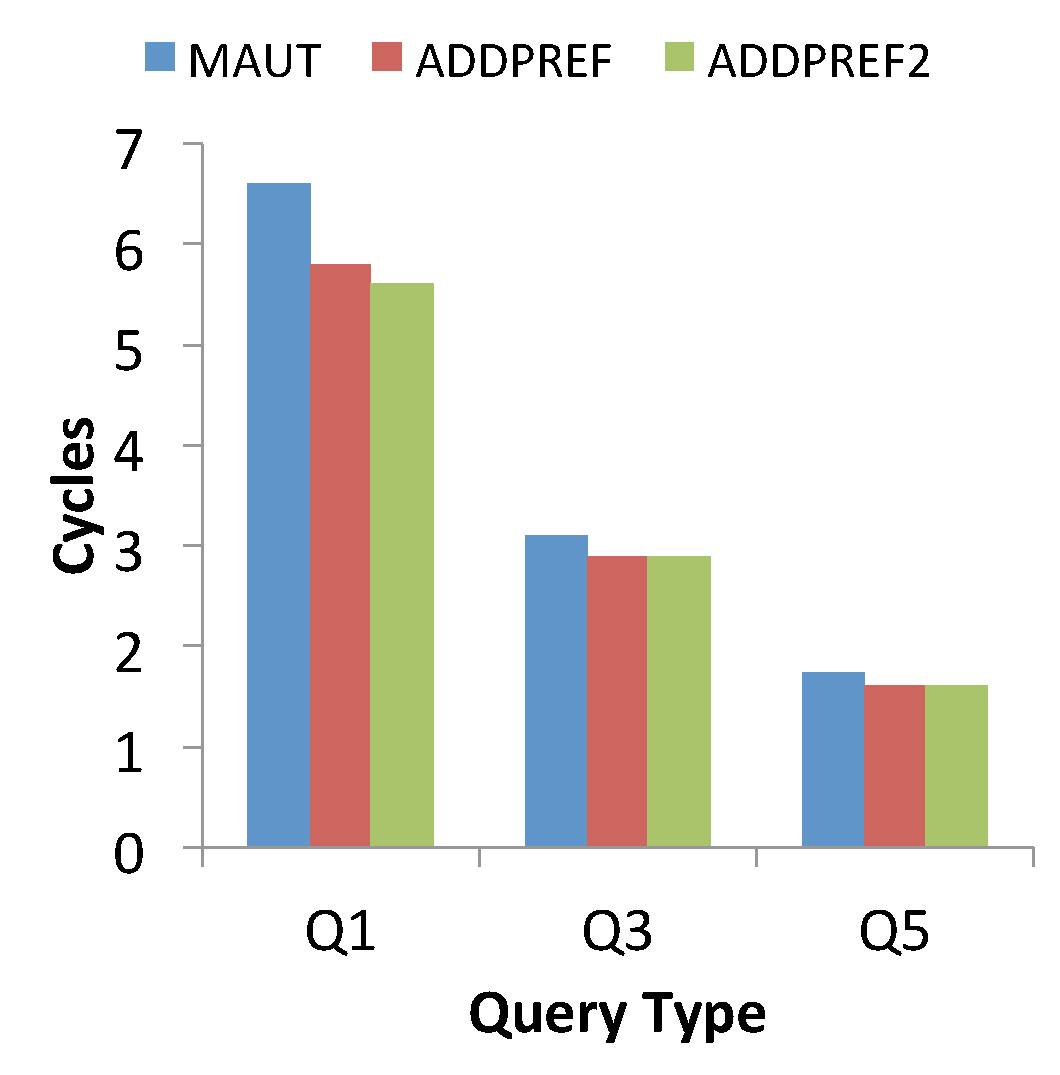
\includegraphics[width=1\linewidth]{figures-bharath/addPref_pc_opt}
  \caption[]{Average number of interaction cycles on PC dataset - optimal user model}
  \label{fig:addPref_pc_opt}
\end{minipage}
\end{figure}

\begin{figure}[h]
\centering
\begin{minipage}{.45\textwidth}
  \centering
  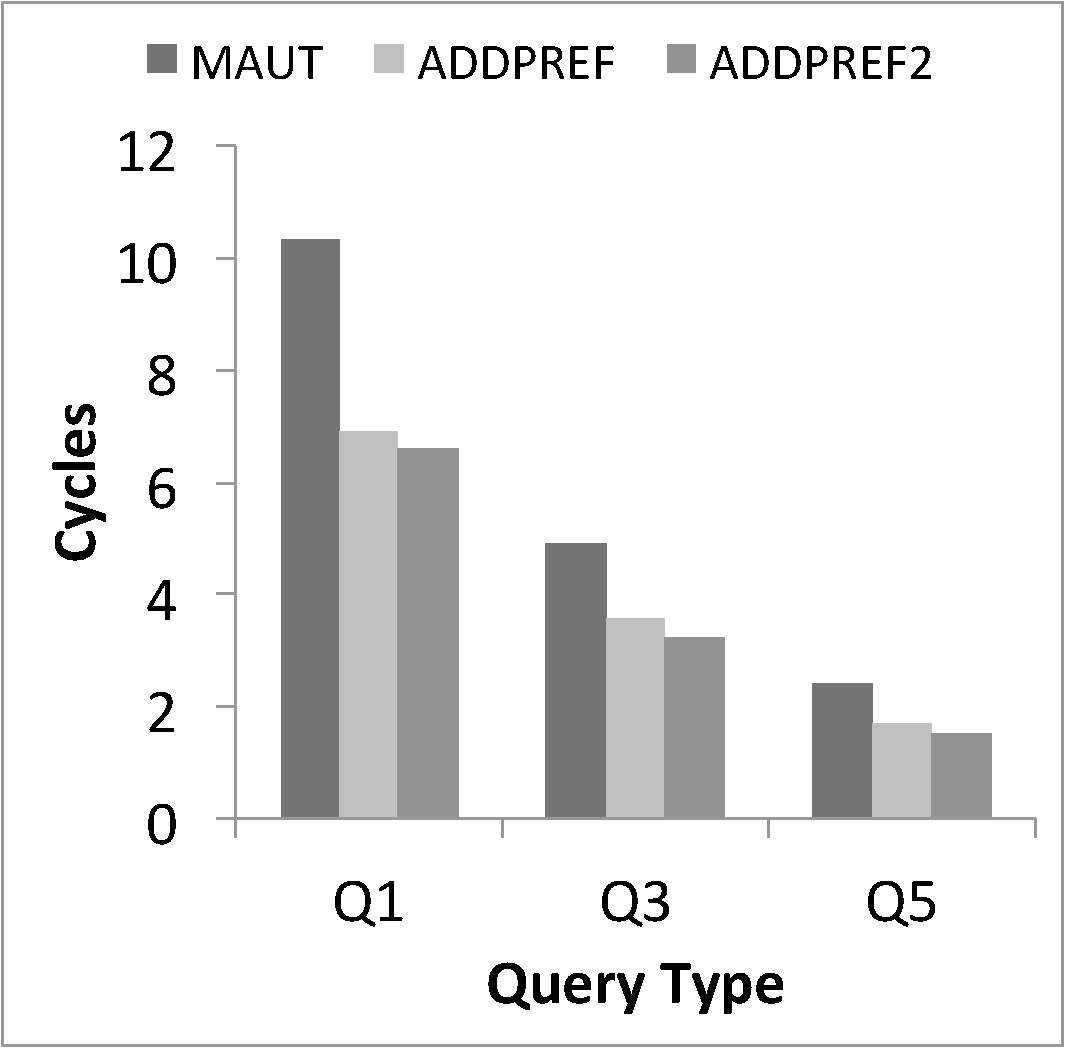
\includegraphics[width=1\linewidth]{figures-bharath/addPref_camera_noisy}
  \caption[]{Average number of interaction cycles on Camera dataset - noisy framework}
  \label{fig:addPref_camera_noisy}
\end{minipage}%
\;\;\;\;\;\;
\begin{minipage}{.45\textwidth}
  \centering
  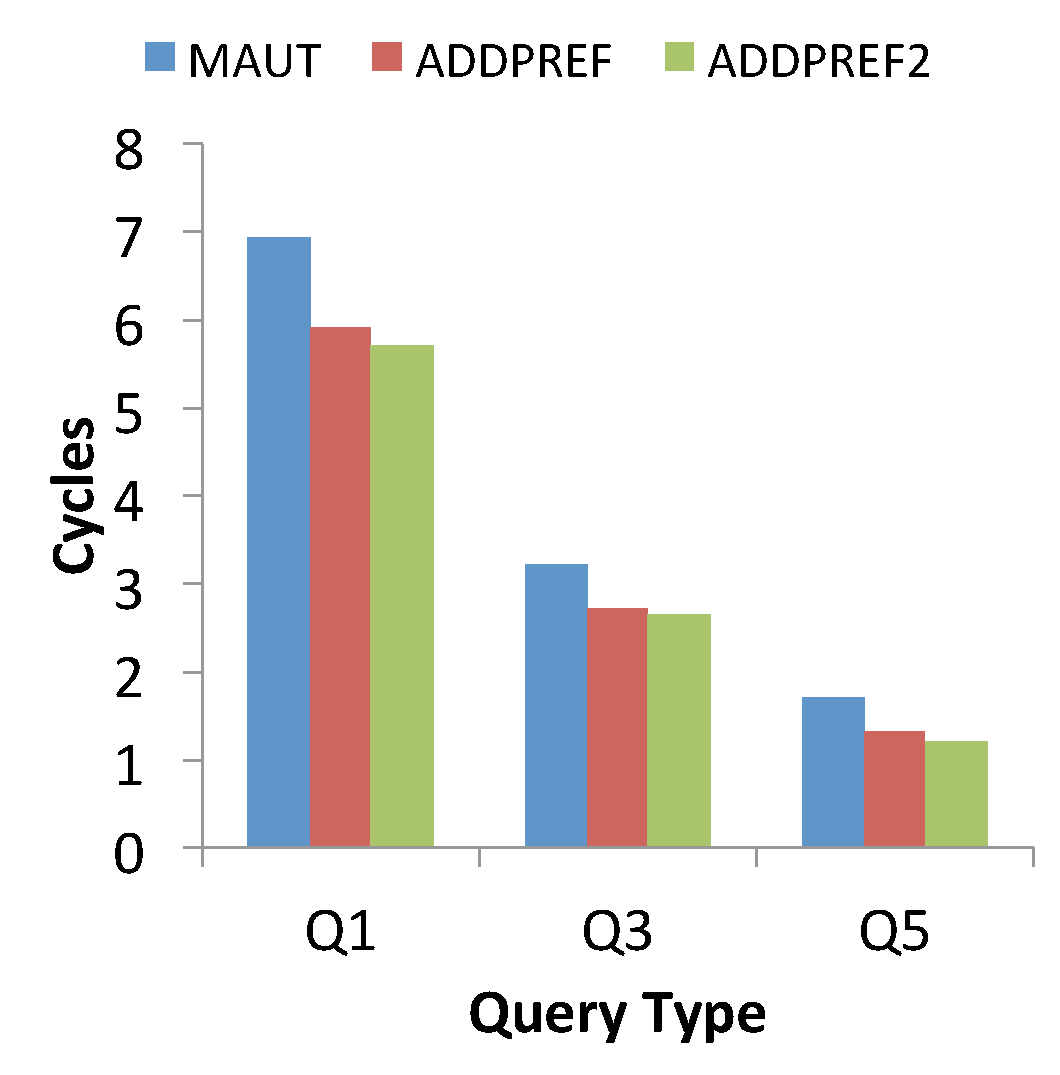
\includegraphics[width=1\linewidth]{figures-bharath/addPref_pc_noisy}
  \caption[]{Average number of interaction cycles on PC dataset - noisy framework}
  \label{fig:addPref_pc_noisy}
\end{minipage}
\end{figure}

In Section \ref{sec:sim}, we have proposed a modification, SIM, where products that are most similar to user's initial query are chosen as the top$K$ products in the first cycle.
This simple modification actually produces a very high improvement in the number of interaction cycles.
For the camera dataset and in optimal setting, SIM reduces the number of cycles by 30.6\% on an average.
SIM when combined with ADDPREF2, reduces the average number of cycles even further. 
The reduction is 40.3\% on average in this case.
%The results obtained in the optimal setting for Camera and PC datasets have been shown in Figures \ref{fig:sim_camera_opt} and \ref{fig:sim_pc_opt}. 
Results for the noisy setting and PC dataset are shown in Table \ref{tab:summary}.

%\begin{figure}[h]
%\centering
%\begin{minipage}{.45\textwidth}
%  \centering
%  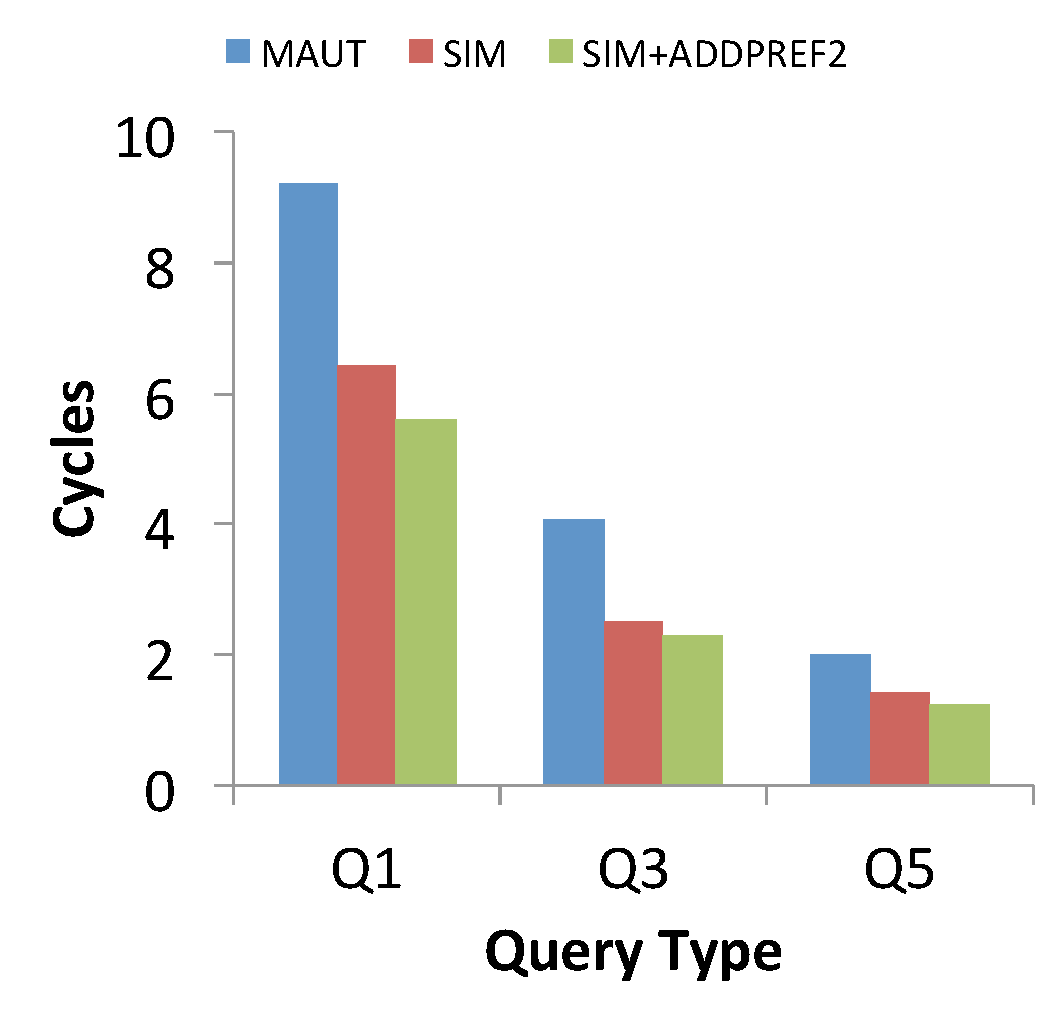
\includegraphics[width=1\linewidth]{figures-bharath/sim_camera_opt}
%  \caption[]{Average number of interaction cycles on Camera dataset - optimal user model}
%  \label{fig:sim_camera_opt}
%\end{minipage}%
%\;\;\;\;\;\;
%\begin{minipage}{.45\textwidth}
%  \centering
%  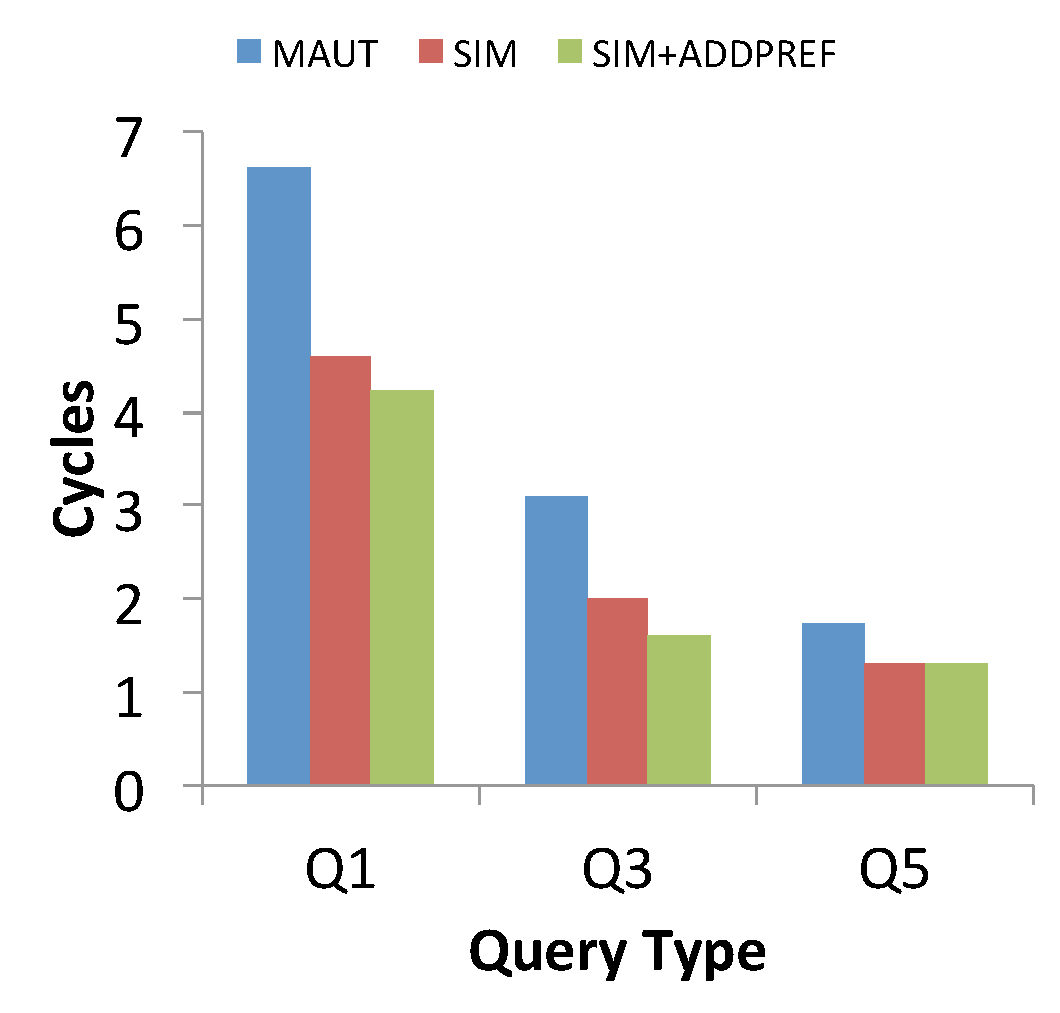
\includegraphics[width=1\linewidth]{figures-bharath/sim_pc_opt}
%  \caption[]{Average number of interaction cycles on PC dataset - optimal user model}
%  \label{fig:sim_pc_opt}
%\end{minipage}
%\end{figure}
\subsection{Algorithms that selectively update weights and value functions of attributes(SELWEIGHT and SELNOMINAL)}
The algorithm SELWEIGHT, described in Section \ref{sec:sel} that updates weights of numeric attributes by examining the critique patterns of selected product and also the $k-1$ rejected products.
SELNOMINAL, described in Section \ref{sec:selNominal} updates value functions by examining the nominal attribute values of the rejected $k-1$ products.
SELWEIGHT and SELNOMINAL take 7.65 and 7.08 cycles respectively for Camera dataset for the queries of type Q1 in an optimal framework.
When both the above algorithms are combined, the resulting algorithm performs better than both the individual algorithms.
The resulting algorithm takes only 6.78 cycles on an average to reach the target product.
MAUT takes 9.21 cycles on an average in this scenario.
%This means that SELWEIGHT and SELNOMINAL can guide the user through the product space very efficiently if the user is not very well aware of the domain.
%The superior performance of both SELWEIGHT and SELNOMINAL is maintained for Q3 as well as Q5 on both the datasets.
The number of interaction cycles taken by these two algorithms is shown in Figures \ref{fig:sel_camera_opt} to \ref{fig:sel_pc_noisy}.
The average improvement achieved by these algorithms in different scenarios is given in Table \ref{tab:summary}.

\begin{figure}[h]
\centering
\begin{minipage}{.45\textwidth}
  \centering
  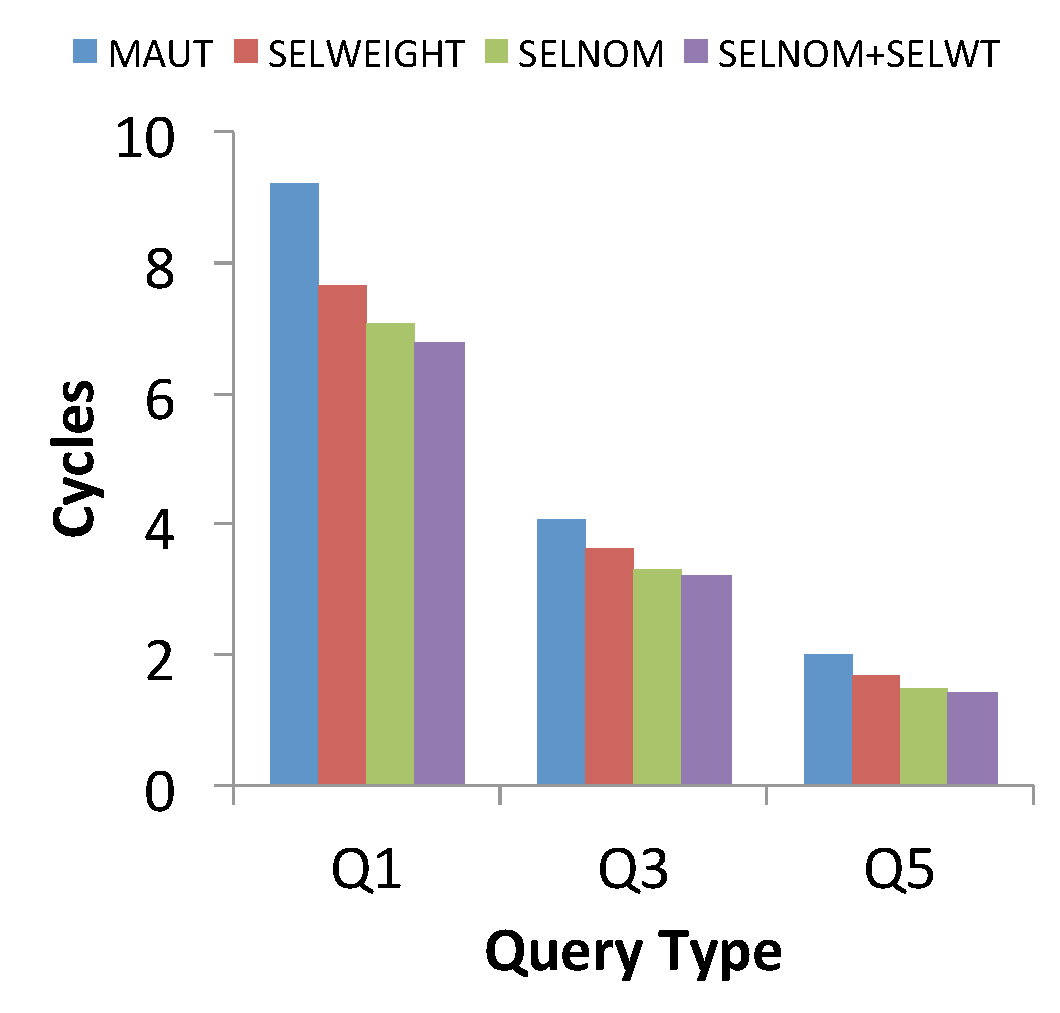
\includegraphics[width=1\linewidth]{figures-bharath/sel_camera_opt}
  \caption[]{Average number of interaction cycles on Camera dataset - optimal user model}
  \label{fig:sel_camera_opt}
\end{minipage}%
\;\;\;\;\;\;
\begin{minipage}{.45\textwidth}
  \centering
  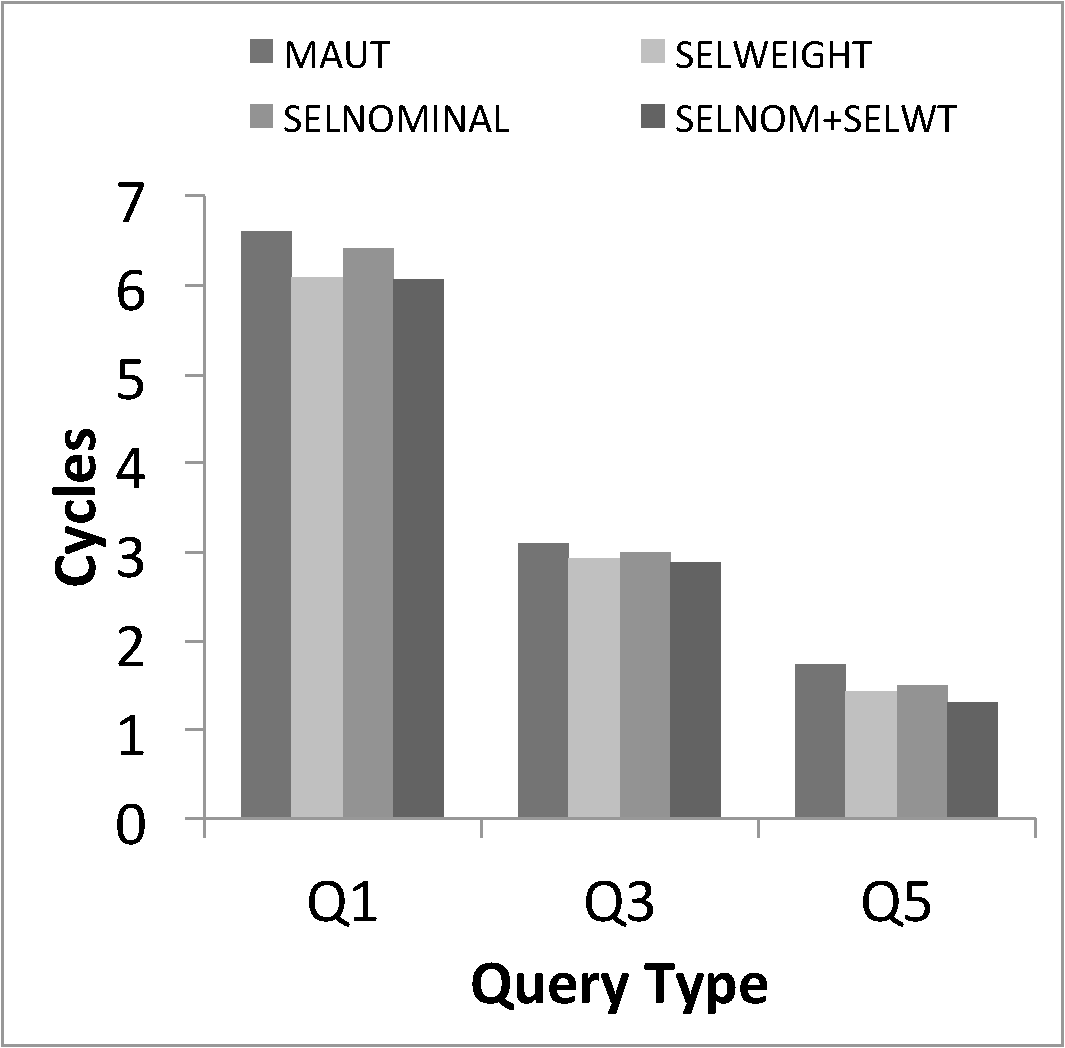
\includegraphics[width=1\linewidth]{figures-bharath/sel_pc_opt}
  \caption[]{Average number of interaction cycles on PC dataset - optimal user model}
  \label{fig:sel_pc_opt}
\end{minipage}
\end{figure}

\begin{figure}[h]
\centering
\begin{minipage}{.45\textwidth}
  \centering
  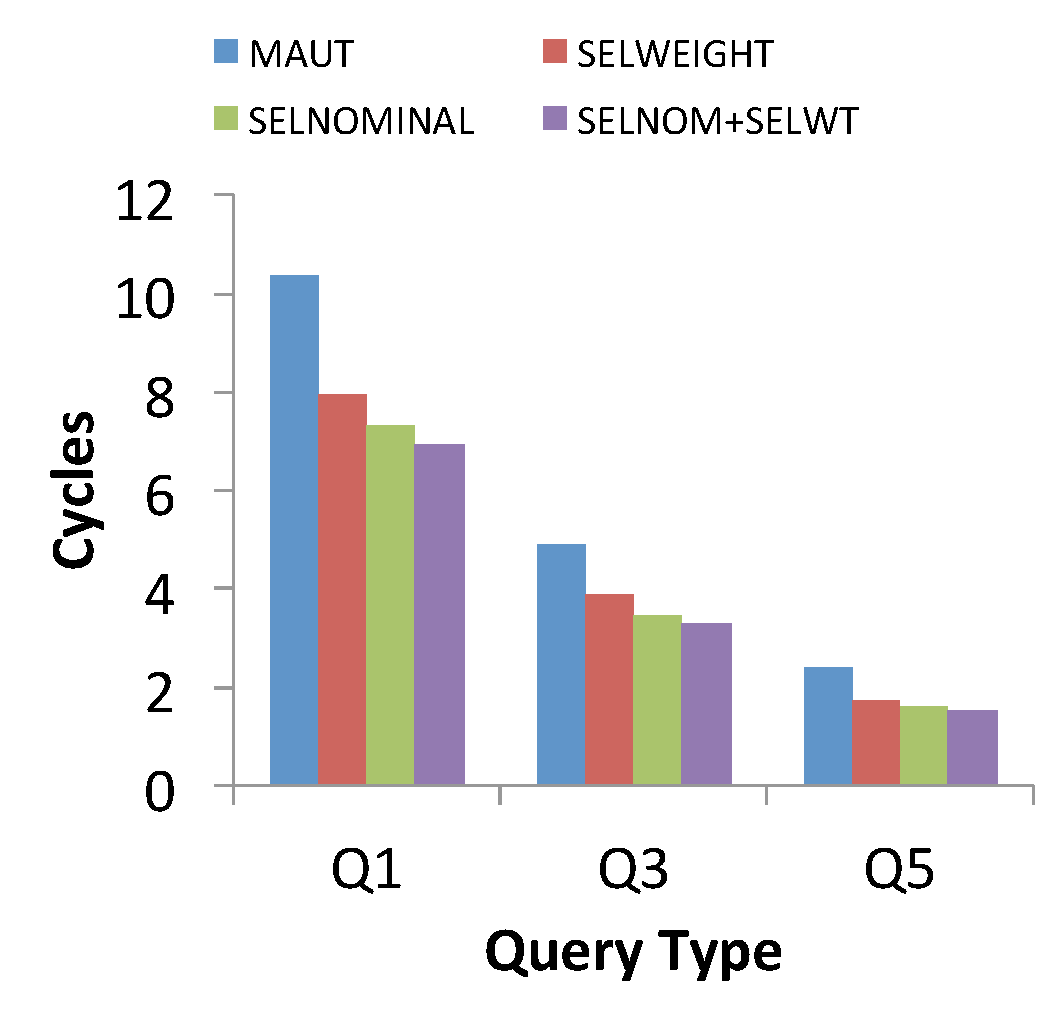
\includegraphics[width=1\linewidth]{figures-bharath/sel_camera_noisy}
  \caption[]{Average number of interaction cycles on Camera dataset - noisy framework}
  \label{fig:sel_camera_noisy}
\end{minipage}%
\;\;\;\;\;\;
\begin{minipage}{.45\textwidth}
  \centering
  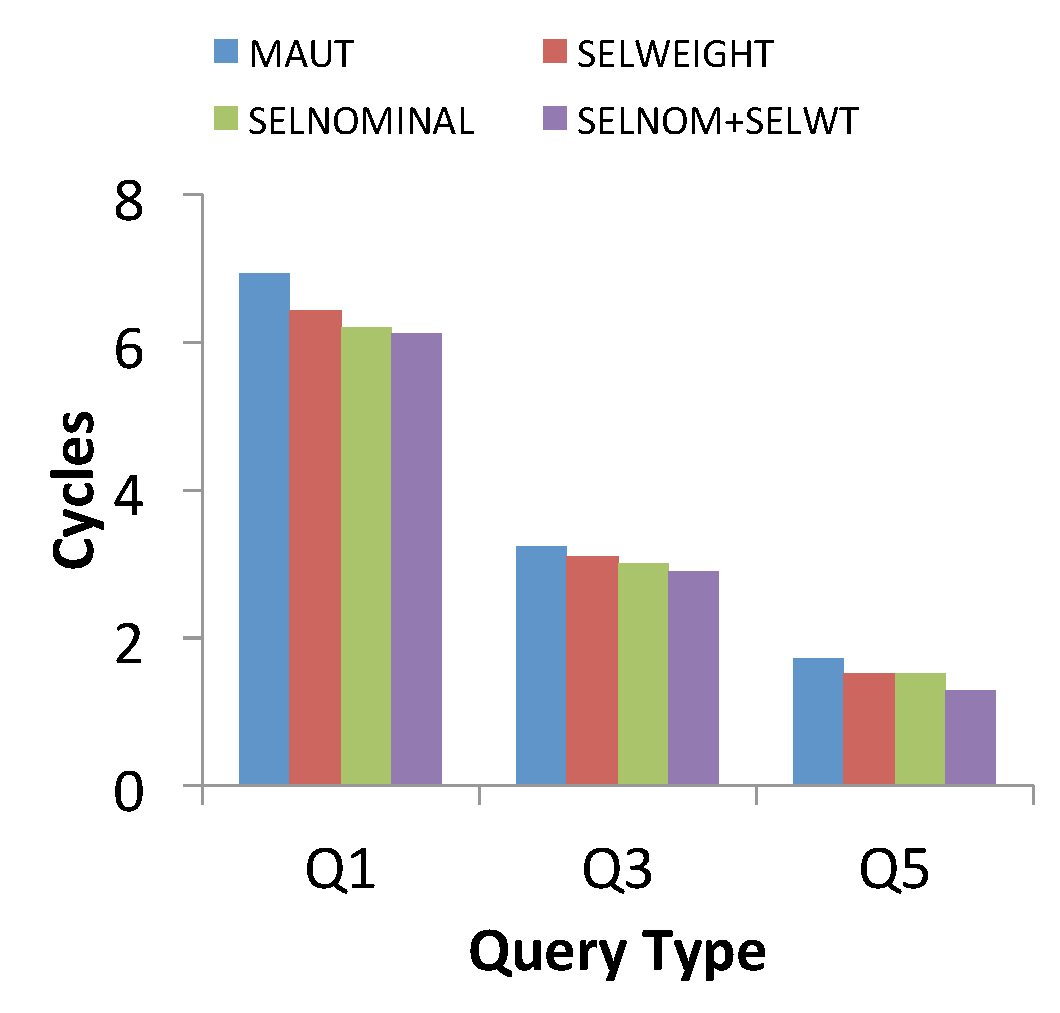
\includegraphics[width=1\linewidth]{figures-bharath/sel_pc_noisy}
  \caption[]{Average number of interaction cycles on PC dataset - noisy framework}
  \label{fig:sel_pc_noisy}
\end{minipage}
\end{figure}


\subsection{Results for the algorithms INIT, HIST, ADD}
The algorithm INIT, described in Section \ref{sec:marketEq} uses the intuition that products which have a high number of dominators with respect to numeric attributes should have nominal attributes with a high value.
If we just change the initialization of value functions of nominal attributes according to this algorithm, we can achieve an improvement of 6\% on an average.
The algorithm HIST, described in Section \ref{sec:hist} updates preference model according to a weighted sum of previously selected products' attributes.
Using HIST, we can achieve an average of 10.3\% on Camera dataset and 4\% improvement on PC dataset.
In Section \ref{sec:hist}, we proposed ADD, an additive model for  updating weights of numeric attributes in each cycle.
The method of updating value functions of nominal attributes remains unchanged.
Using ADD, we can achieve an average of 7.2\% on Camera dataset and 5.7\% improvement on PC dataset.
The algorithm ADD can be used in conjunction with any of the other improvements described in Chapter \ref{chap:modifications} to get slightly better performance.
The performance of the above three algorithms in different scenarios with PC and Camera datasets is shown in Figures \ref{fig:finalMix_camera_opt} to \ref{fig:finalMix_pc_noisy}.

\begin{figure}[h]
\centering
\begin{minipage}{.45\textwidth}
  \centering
  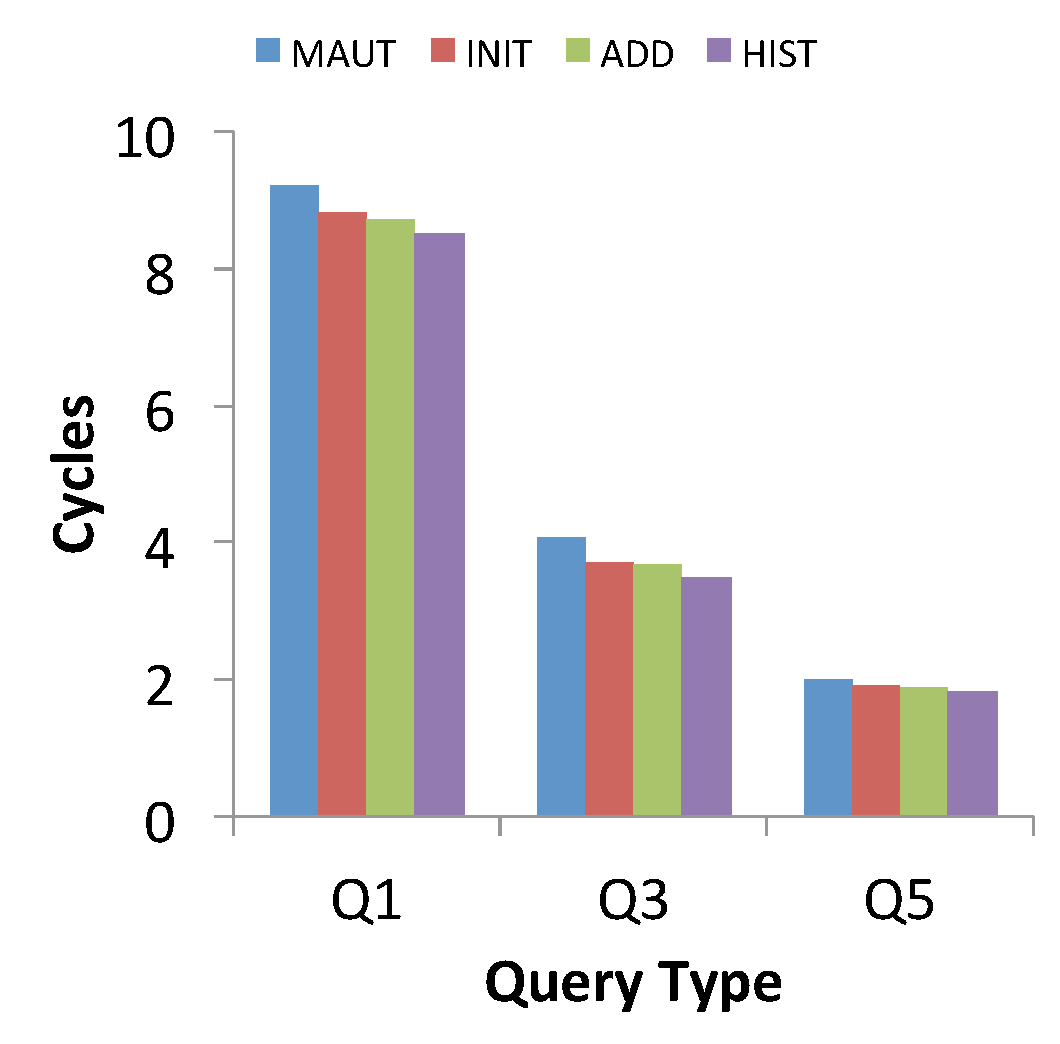
\includegraphics[width=1\linewidth]{figures-bharath/finalMix_camera_opt}
  \caption[]{Average number of interaction cycles on Camera dataset - optimal user model}
  \label{fig:finalMix_camera_opt}
\end{minipage}%
\;\;\;\;\;\;
\begin{minipage}{.45\textwidth}
  \centering
  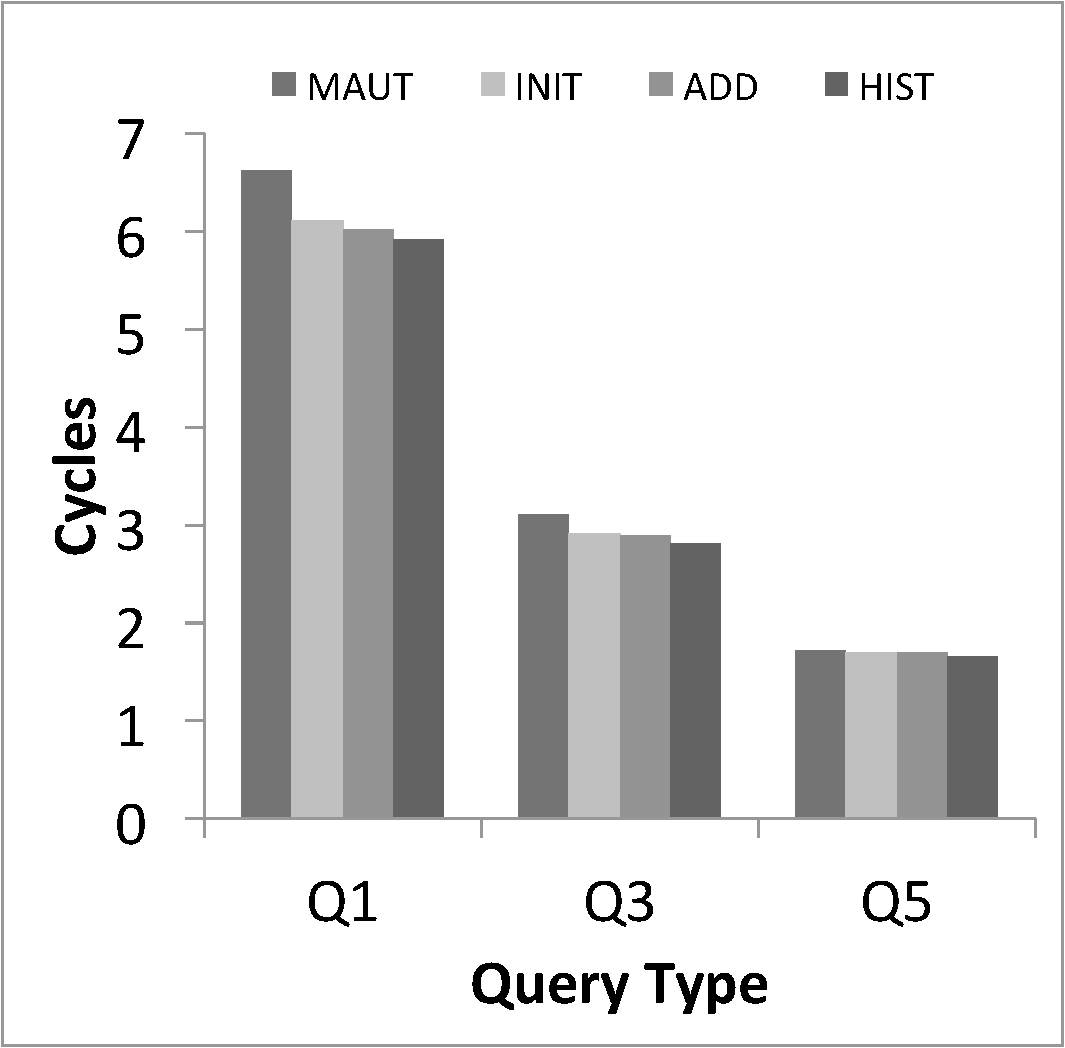
\includegraphics[width=1\linewidth]{figures-bharath/finalMix_pc_opt}
  \caption[]{Average number of interaction cycles on PC dataset - optimal user model}
  \label{fig:finalMix_pc_opt}
\end{minipage}
\end{figure}

\begin{figure}[h]
\centering
\begin{minipage}{.45\textwidth}
  \centering
  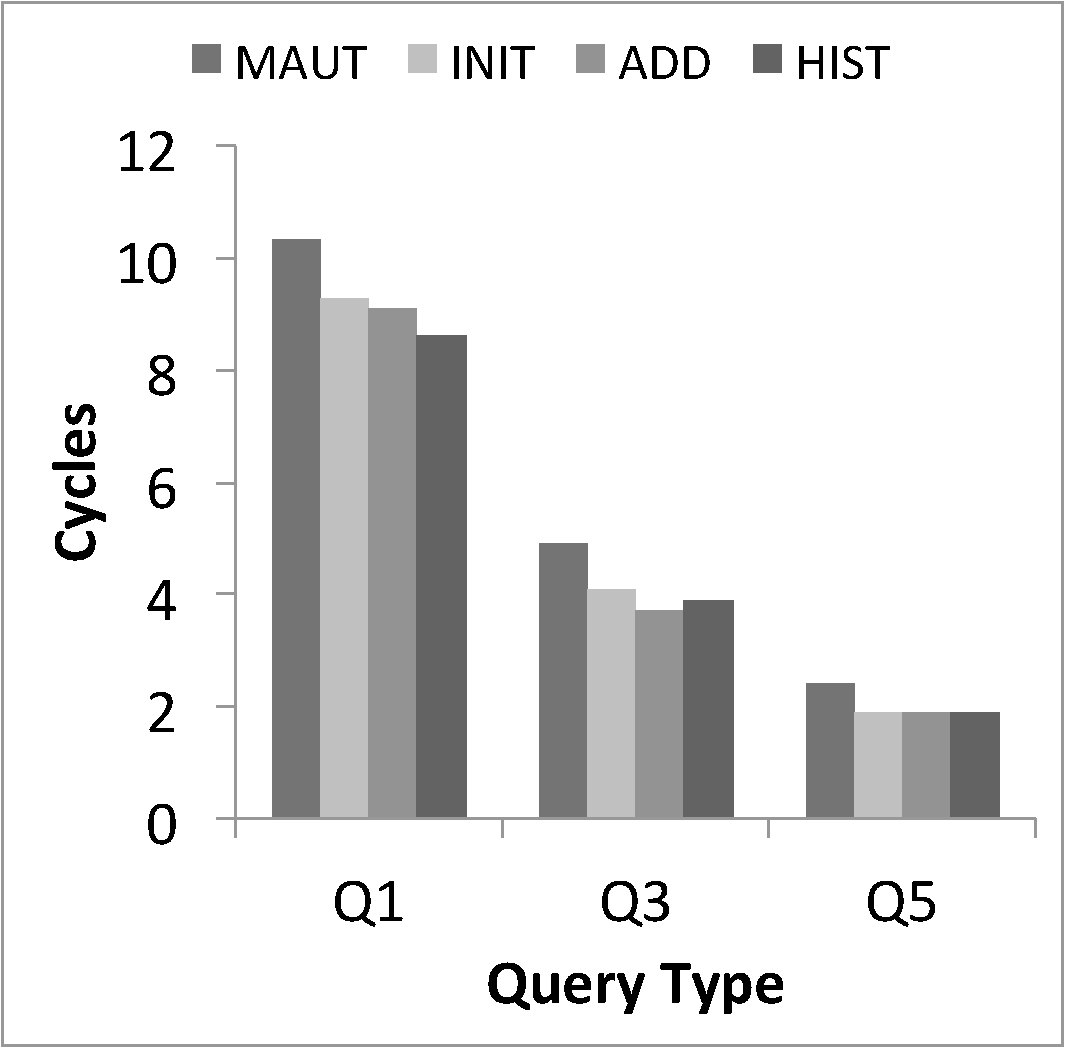
\includegraphics[width=1\linewidth]{figures-bharath/finalMix_camera_noisy}
  \caption[]{Average number of interaction cycles on Camera dataset - noisy framework}
  \label{fig:finalMix_camera_noisy}
\end{minipage}%
\;\;\;\;\;\;
\begin{minipage}{.45\textwidth}
  \centering
  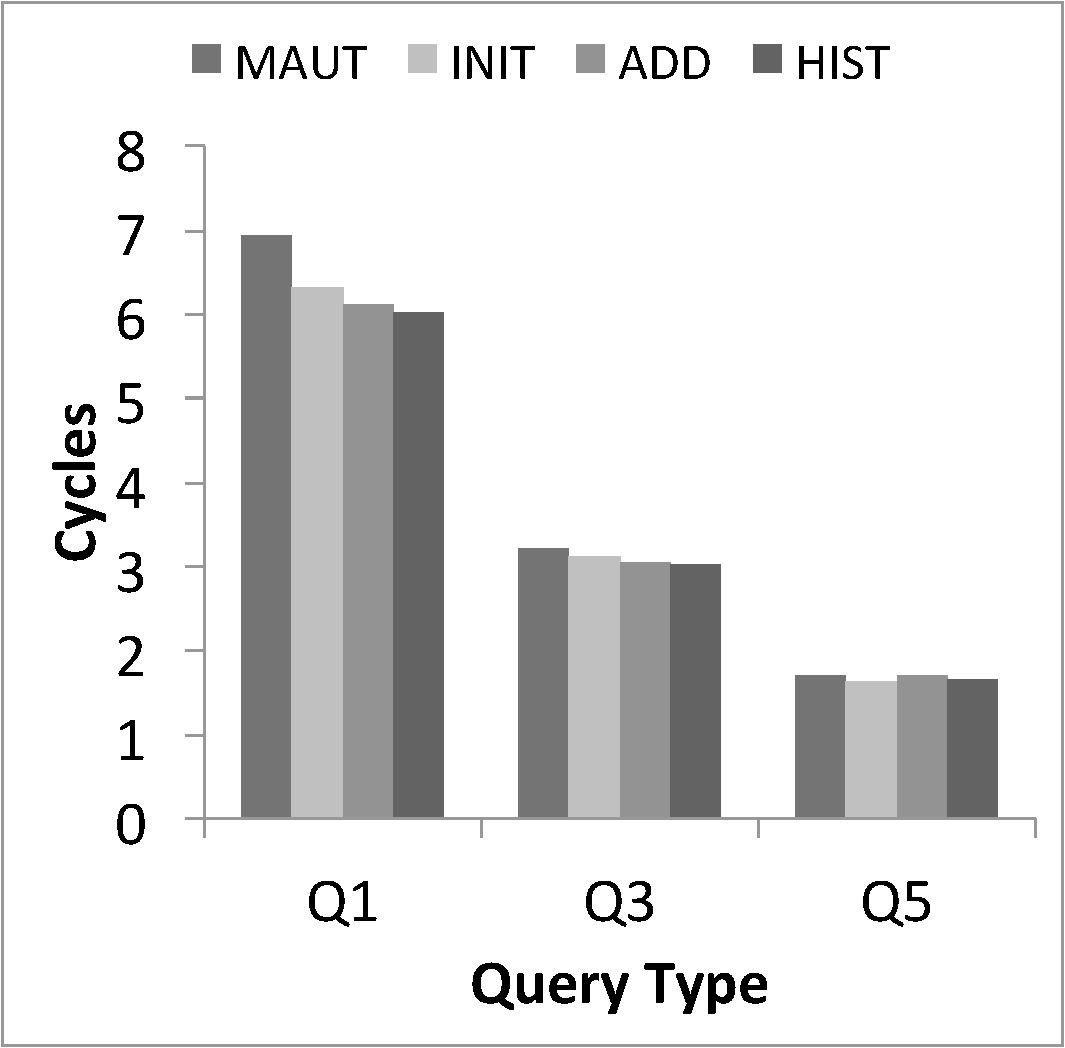
\includegraphics[width=1\linewidth]{figures-bharath/finalMix_pc_noisy}
  \caption[]{Average number of interaction cycles on PC dataset - noisy framework}
  \label{fig:finalMix_pc_noisy}
\end{minipage}
\end{figure}



\begin{table}
\caption{Summary of experimental results}
\centering
\renewcommand{\arraystretch}{1.2}
\label{tab:summary}

\begin{tabular}{|p{3.5cm}|p{1.8cm}|p{1.9cm}|p{1.9cm}|p{1.9cm}|}
 \cline{1-5}
 & &\multicolumn{3}{c|}{\% improvement in number of interaction cycles}\\
 \cline{1-5}

Algorithm & Camera-OPT & Camera-Noisy & PC-OPT & PC-Noisy \\
 \cline{1-5}
DIV & 22.6  &29.5 &10.3 &18.9\\
\hline
DIV2 &27.9 &38.8 &11.4 &21.6\\
\hline
SELWEIGHT &14.8 &24.4 &10.5 &7.8\\
\hline
SELNOMINAL &22.2 &30.8 &12.3 &9.5\\
\hline
SELWEIGHT + SELNOMINAL &25.6 &34.5 &13.1 &15.1\\
\hline
ADDPREF &29.1 &29.9 &8.34 &17.6\\
\hline
ADDPREF2 &33.7 &36.1 &9.49 &21.6\\
\hline
SIM &30.6 &37.6 &29.8 &24.6\\
\hline
SIM + ADDPREF2 &40.3 &45.3 &26.2 &33.8\\
\hline
INIT &6.12 &10.1 &5.3 &5.7\\
\hline
ADD &7.2 &19.2 &5.7 &5.9\\
\hline
HIST &10.3 &19.4 &3.9 &4.5\\
\hline





\hline
\end{tabular}
\end{table}

